\section{Flow around a cube matrix}
\label{sec_cube_matrix}

In this section a flow around the cube matrix is solved using Direct Numerical
Simulation (DNS). It is a DNS in sense that not sub-grid-scale (SGS) model is
used, rather in the sense that it resolves {\em all} scales of motion. 
Cube matrix is placed at the bottom of the plane channel. The flow is
assumed to be fully developed, so it only suffices to simulate one flow
segment (flow around one cube) with periodic boundary conditions applied in
stream-wise~($x$) and span-wise~($y$) direction. Problem domain is illustrated
in Fig.~\ref{fig_matrix_domain}. The dimensions of the problem domain are
as follows: $D=6 \, [cm]$, $H=5.1 \, [cm]$ and $h=1.5 \, [cm]$. Working
fluid is air, having density $\rho = 1.205 \, [kg/m^3]$ and kinematic
viscosity~$\nu = 1.511 \times 10^{-5}$.

%-------------------%
%                   %
%  Matrix of cubes  %
%                   %
%-------------------%
\begin{figure}[ht]
  \centering
  \setlength{\unitlength}{1mm}
  \begin{picture}( 66, 44)(0,0)
    \thickbox{ 66}{ 44}
    \put(0,0){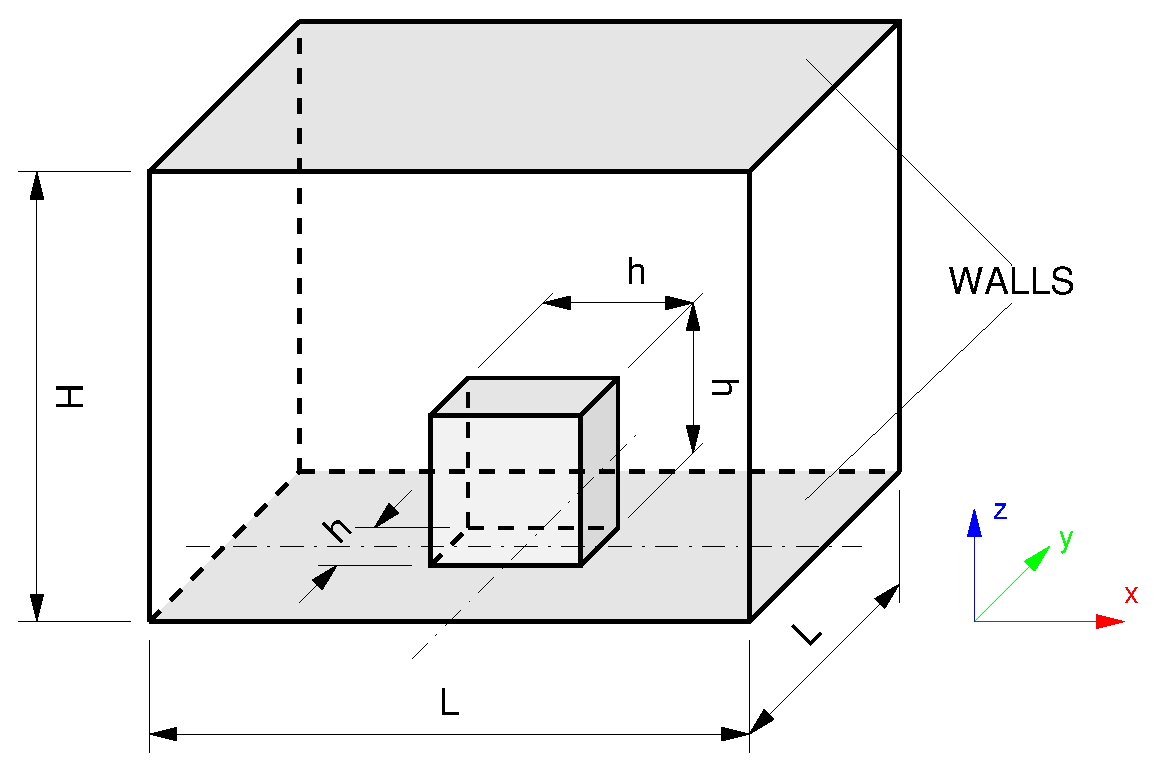
\includegraphics[scale=0.35]{Figures/09-03-matrix-gray.eps}}
  \end{picture}
  \caption{Problem domain for the flow around a cube matrix.} 
  \label{fig_matrix_domain}
\end{figure}

Flow rate for this case is specified with stream-wise bulk velocity equal 
to~$u_b = 3.86 \, [m/s]$. Reynolds number based on channel height 
is~$Re \approx 13000$. At this~$Re$, the flow is turbulent. This case,
in fact, is the first simulation of a turbulent flow in this tutorial.
{\psiboil} is a tool which simulates turbulent flows using Large Scale
Simulation (LSS) approaches, namely the DNS and LES\footnote{In more
general sense, LSS includes also simulation of turbulent flows with
interface tracking, but as it is still an active area of research,
nomenclature is not yet fully established.} 

Simulation of turbulent flows with LES/DNS consists of two steps:
%
\begin{itemize}
  \item Unsteady flow simulation
  \item Computation of flow statistics
\end{itemize}
%
First step generates a sequence of unsteady flow realizations stored on
a disk, while the second step reads the flow realizations from disk and
computes necessary statistics (Reynolds stresses, turbulent kinetic
energy, correlation, turbulent spectra, etc.). Having {\psiboil}'s
philosophy in mind\footnote{It is not an integral package suited for 
all flow situations one can encounter, but rather a suite of objects which 
facilitates building of different algorithms for flow simulation.} two
different programs will be outlined in this section: one for
unsteady flow simulation {\tt 09-03-main.cpp} and the other for
computation of flow statistics {\tt 09-03-stat.cpp}. Obviously these
two codes share some object definitions. The shared objects are stored
in {\tt C++} header file {\tt 09-03-common.h}.

\subsection{Unsteady flow simulation}
\label{sub_sec_unsteady_flow}

The program which conducts the unsteady flow simulation is very similar
to program introduced in~Sec.~\ref{sec_cylinder}. It also follows 
closely the typical {\psiboil} program layout introduced in Chap.~\ref{chap_structure}.

To compile it, you do not only need a link to {\em main} program in
{\em source} directory ({\tt PSI-Boil/Src}), but also to the include 
file~({\tt 09-03-common.h}). You can get the main program and the include 
file, provided you are in source directory, with:
%
\begin{verbatim}
> ln -i -s ../Doc/Tutorial/Volume1/Src/09-03-main.cpp main.cpp
> ln -i -s ../Doc/Tutorial/Volume1/Src/09-03-common.h .
\end{verbatim} 
%
The include file holds grids and domain definition, and is included in the 
main program with the:
%
{\small \begin{verbatim}
     13   #include "09-03-common.h"
\end{verbatim}}
%
There is nothing new in these definitions, so there is no need to
explain them in more detail here. {\tt Times} object is defined in
line:
%
{\small \begin{verbatim}
     16   Times time(100000, 0.00002); /* ndt, dt */
\end{verbatim}}
%
For an LSS, we do not expect to get a steady solution to the problem.
We are aware (and hopeful) that simulation will yield an unsteady
solution and we want to perform enough time steps to get a relevant
statistical sample for later computation of flow statistics. Here 
we set the number of time step to~$100000$. Time step which gives 
the~CFL number in the stable range~($0.3-0.4$) is $0.00002$. The
physical time of this simulation is thus $2 \, [s]$.

The program defines variables (velocity, pressure and their sources)
in lines~21--22. Boundary conditions for variables are set in lines~24--38.
That is followed by the definition of materials (lines~43--45),
solver (line~47), transport equations (lines~52 and~53). As usually,
multigrid solver is defined for pressure equation (in line~59).
For this case, the flow is not initialized, but the forces in momentum
equations are (lines~61 and~62). 

The time loop, which spans from lines~67--105, has all the steps
introduced before, say in~Sec.~\ref{sec_cylinder}, but it has a
small section which re-computes the pressure drop at each time 
step to keep the bulk velocity constant, and a section which 
periodically saves the data for later computations of flow
statistics.

Mass flow in computational domain is kept constant using the second
Newton's law:
%
\be
  F = m \cdot a \; \; \; \; [N]
\ee
%
If applied to a computational domain, acceleration $a$ is the rate
of change of bulk velocity. Force~$F$, on the other hand is integrated
pressure drop in the domain. Hence, second Newton's law, can be
written as:
%
\be
  \frac{\p p^n}{\p x} V 
  =
  m \cdot \frac{u_b^n - u_b^{n-1}}{\Delta t} \; \; \; \; [N]
\ee
%
We want the bulk velocity at new time step~($u_b^n$) to be equal to
the prescribed (desired) bulk velocity~($u_{des}$). Furthermore,
acknowledging that mass~$m$ divided by volume~$V$ is density, the
expression for pressure drop which gives the desired bulk velocity
in the new time step is:
%
\be
  \frac{\p p^n}{\p x} 
  = 
  \rho \cdot \frac{u_{des} - u_b^{n-1}}{\Delta t} 
  \label{eq_newton_second}
\ee
%
The implementation of this expression is given in lines~91--96.
%
{\small \begin{verbatim}
     91     real b_new = ns.bulk(Comp::u(), LX*0.333);
     92
     93     real p_drop = fluid.rho() * (b_des - b_new) / time.dt();
     94
     95     Comp m = Comp::u();
     96     for_vmijk(xyz,m,i,j,k) xyz[m][i][j][k] = p_drop * uvw.dV(m,i,j,k);
\end{verbatim}}
%
Line~91 computes bulk velocity in~$x$ direction using {\tt Momentum}'s
member function {\tt bulk}. As the parameter, this function takes the
desired component ({\tt Comp}) and the~$x$ coordinate at which the bulk 
velocity is computed\footnote{Although
it should be the same at any position.}. Line~93 is the implementation
of~Eq.~\ref{eq_newton_second}, while lines~95 and~96 insert new pressure
drop to the momentum equation.

Periodic savings of turbulent velocity fields are performed in line:
%
{\small \begin{verbatim}
    102     if( time.current_step() % 50 == 0 ) uvw.save("uvw", time.current_step());
\end{verbatim}}
%
The line~102 checks the reminder of division of the current time step
with~50, and if it is zero, velocity is saved in the binary
format, using the {\tt Vector}'s member function {\tt save}. This
member function is available for {\tt Scalar}s as well. The {\tt save}
functions just dumps the memory occupied by a certain field variable
into a binary file. As such, it can not be visualized with a post-processing
tool. The {\tt save} command saves the files with extension~{\tt .bck} 
(to remind of {\em backup}).
As with other {\psiboil} output function, even here each processors
writes it's own file but they can {\em not} be connected into a single
one using the {\tt Connect} program.

Lines~103 and~104:
%
{\small \begin{verbatim}
    103     if( time.current_step() % 5000 == 0) /* 5000 */
    104       boil::plot->plot(uvw,p,"uvw,p", time.current_step());
\end{verbatim}}
%
store variables (velocity and pressure) for post-processing each
5000 time steps. Examples of these unsteady flow fields (realizations)
are given in~Fig.~\ref{fig_matrix_velocity}.

%------------%
%            %
%  Velocity  %
%            %
%------------%
\begin{figure}
  \centering
  \setlength{\unitlength}{1mm}
  \begin{picture}(145,195)(0,0)
    \thickbox{145}{195}
    \put( -3,153){\includegraphics[width=4.8cm]{Figures/09-03/plane_xy_20000.eps}}
    \put( -3,103){\includegraphics[width=4.8cm]{Figures/09-03/plane_xz_20000.eps}}
    \put(  0,150){$z=7.5 \, [mm]$,  $t=0.4 \, [s]$}
    \put(  0,103){$y=30  \, [mm] $, $t=0.4 \, [s]$}

    \put( 47,153){\includegraphics[width=4.8cm]{Figures/09-03/plane_xy_40000.eps}}
    \put( 47,103){\includegraphics[width=4.8cm]{Figures/09-03/plane_xz_40000.eps}}
    \put( 50,150){$z=7.5 \, [mm]$,  $t=0.8 \, [s]$}
    \put( 50,103){$y=30  \, [mm] $, $t=0.8 \, [s]$}

    \put( 97,153){\includegraphics[width=4.8cm]{Figures/09-03/plane_xy_60000.eps}}
    \put( 97,103){\includegraphics[width=4.8cm]{Figures/09-03/plane_xz_60000.eps}}
    \put(100,150){$z=7.5 \, [mm]$,  $t=1.2 \, [s]$}
    \put(100,103){$y=30  \, [mm] $, $t=1.2 \, [s]$}

    \put( -3, 53){\includegraphics[width=4.8cm]{Figures/09-03/plane_xy_80000.eps}}
    \put( -3,  3){\includegraphics[width=4.8cm]{Figures/09-03/plane_xz_80000.eps}}
    \put(  0, 50){$z=7.5 \, [mm]$,  $t=1.6 \, [s]$}
    \put(  0,  3){$y=30  \, [mm] $, $t=1.6 \, [s]$}

    \put( 47, 53){\includegraphics[width=4.8cm]{Figures/09-03/plane_xy_100000.eps}}
    \put( 47,  3){\includegraphics[width=4.8cm]{Figures/09-03/plane_xz_100000.eps}}
    \put( 50, 50){$z=7.5 \, [mm]$,  $t=2 \, [s]$}
    \put( 50,  3){$y=30  \, [mm] $, $t=2 \, [s]$}

    \put( 97, 53){\includegraphics[width=4.8cm]{Figures/09-03/plane_xy_mirror_100000.eps}}
    \put( 97,  3){\includegraphics[width=4.8cm]{Figures/09-03/plane_xz_mirror_100000.eps}}
    \put(100, 50){$z=7.5 \, [mm]$,  time averaged}
    \put(100,  3){$y=30  \, [mm] $, time averaged}
  \end{picture}
  \caption{Unsteady and time-averaged velocity fields colored by the magnitude of 
           stream-wise~($x$) velocity component.}
  \label{fig_matrix_velocity}
\end{figure}

\subsection{Computation of flow statistics}
\label{sub_sec_flow_statistics}

Program for computation of flow statistics~({\tt 09-03-stat.cpp}) does not
follow the typical {\psiboil}'s program structure. Therefore, it is given
and explained here in full detail. 
%
{\small \begin{verbatim}
      1 #include "Include/psi-boil.h"
      2
      3 #include <vector>
      4
      5 /****************************************************************************/
      6 main(int argc, char * argv[]) {
      7
      8   boil::timer.start();
      9
     10   /*------------------------------+
     11   |  grids, obstacles and domain  |
     12   +------------------------------*/
     13   #include "09-03-common.h"
     14
     15   /*------------------+
     16   |  define unknowns  |
     17   +------------------*/
     18   Vector uvw(d);   // velocity
     19   Scalar ut(d);  Scalar vt(d);  Scalar wt(d);     // temporary u, v, w
     20   Scalar u (d);  Scalar v (d);  Scalar w (d);     // averaged  u, v, w
     21   Scalar uu(d);  Scalar vv(d);  Scalar ww(d);     // averaged  uu,vv,ww
     22   Scalar uv(d);  Scalar uw(d);  Scalar vw(d);     // averaged  uv,uw,vw
     23
     24   u  = 0; v  = 0; w  = 0;
     25   uu = 0; vv = 0; ww = 0;
     26   uv = 0; uw = 0; vw = 0;
     27
     28   /* timer */
     29   Times time(80000, 0.00002); /* ndt, dt */
     30   time.first_step(20000);
     31
     32   /*------------+
     33   |  time loop  |
     34   +------------*/
     35   real count = 0;
     36
     37   const Comp U = Comp::u();
     38   const Comp V = Comp::v();
     39   const Comp W = Comp::w();
     40
     41   for(time.start(); time.end(); time.increase()) {
     42
     43     /*-------+
     44     |  load  |
     45     +-------*/
     46     if( time.current_step() % 100 == 0 ) {
     47       boil::oout << "##########################" << boil::endl;
     48       boil::oout << "# GETTING TIME STEP: " << time.current_step() << boil::endl;
     49       boil::oout << "#-------------------------" << boil::endl;
     50
     51       count ++;
     52
     53       uvw.load("uvw", time.current_step());
     54
     55       for_vijk(u,i,j,k) {
     56         ut[i][j][k] = 0.5 * (uvw[U][i][j][k] + uvw[U][i+1][j]  [k]  );
     57         vt[i][j][k] = 0.5 * (uvw[V][i][j][k] + uvw[V][i]  [j+1][k]  );
     58         wt[i][j][k] = 0.5 * (uvw[W][i][j][k] + uvw[W][i]  [j]  [k+1]);
     59       }
     60
     61       u  += ut;     v  += vt;     w  += wt;
     62       uu += ut*ut;  vv += vt*vt;  ww += wt*wt;
     63       uv += ut*vt;  uw += ut*wt;  vw += vt*wt;
     64     }
     65   }
     66
     67   u  /= count;  v  /= count;  w  /= count;
     68   uu /= count;  vv /= count;  ww /= count;
     69   uv /= count;  uw /= count;  vw /= count;
     70
     71   uu -= u*u;  vv -= v*v;  ww -= w*w;
     72   uv -= u*v;  uv -= u*v;  vw -= v*w;
     73
     74   /*-------+
     75   |  plot  |
     76   +-------*/
     77   boil::plot->plot(u, v, w,   "velocity-mean", time.current_step()-1);
     78   boil::plot->plot(uu,vv,ww,  "stresses-mean", time.current_step()-1);
     79
     80   boil::timer.stop();
     81   boil::timer.report();
     82 }
\end{verbatim}}
%
This program includes the same file ({\tt 09-03-common.h}) as the program for 
unsteady flow simulation to ensure that grids and domains are the same. Fields
for unknowns are defined in lines~18--22. The {\tt Vector uvw} is defined
to loading the results generated in previous step, and~12 more scalars which 
follow will hold temporary (unsteady) velocity components ({\tt ut}, {\tt vt}, {\tt wt}),
time-averaged velocity components ({\tt u}, {\tt v}, {\tt w}) and Reynolds
stress components ({\tt uu}, {\tt vv}, \dots {\tt vw}). The {\tt Scalar}
field which are used for accumulating statistics are initialized in lines~24--26.

Line~29 defines the {\tt Timer}, but contrary to the previous program, it
will execute {\em only} 80000 time steps. However, the time stepping does
not start from zero, but from time step~20000, stipulated in line~30. By
doing so, we will discard first 20000 time steps (corresponding to $0.4 \, [s]$
physical time), thus gather statistics from the time when the flow is already 
fully developed\footnote{Actually, a much more concise procedure would be
needed to ensure this, but it is beyond the scope of this tutorial.}. 

{\tt real} variable~{\tt count} is defined and initialized in line~35. It stores
the number of samples (flow field realizations) used in the computation of
statistics. 

Time loop starts at line~41. This loop increases the counter in line~51 
and then reads the results performed in previous
simulation (program {\tt 09-03-main.cpp}) in line~53. {\tt Vector}'s member
function~{\tt load} is used to read the results and it does exactly the opposite
from {\tt save}: it reads the binary data stored in the {\tt .bck} file and
loads it directly into variable's memory space. This line will work properly 
only if the program is executed {\em on the same number of processors} as the 
simulation program was. 

Once the {\tt Velocity} field is loaded into {\tt uvw} field variable, it is
interpolated into three {\tt Scalar} fields in lines~55--59. {\tt Scalar} 
fields {\tt u}, {\tt v} and {\tt w} hold the unsteady velocity field components,
which are added into mean ones in line~61, and to variables which will hold
Reynolds stresses in lines~62 and~63. For the mean velocity components, simple 
addition is performed, while for the Reynolds stress variables appropriate 
multiplications are added. When the time loop ends (after line~65) these values 
are normalized by the number of samples~(lines~67--69) and Reynolds stresses are
finally computed in lines~71 and~72. 

The procedure for computation of Reynolds stresses might need more explanation.
A Reynolds stress component ($\ol{u'u'}$, for instance), at specified 
position is defined as:
%
\be
  \ol{u'u'} = \frac{1}{T} \int_T u'(t) u'(t) dt
  \label{eq_rs_def}
\ee
%
where over-bar denotes time-averaged value, $T$ is the period of time averaging 
and $u'(t)$ is velocity fluctuation defined as: 
%
\be
  u'(t) = u(t) - \ol{u}
  \label{eq_u_fluct_def}
\ee
%
where $u(t)$ is the magnitude of velocity component at time~$t$, 
while~$\ol{u}$ is the time-averaged velocity component defined as:
%
\be
  \ol{u} = \frac{1}{T} \int_T u(t) dt
\ee
%
What we really compute in line~56, and what we finally have after line~59 
is actually:
%
\be
  \ol{uu} = \int_T u(t) u(t) dt
  \label{eq_UU_def}
\ee
%
The relation between $\ol{u'u'}$ (which we want) and $\ol{uu}$ 
(which we can compute from flow realizations) can be obtained if definition 
of~$u'(t)$ (Eq.~\ref{eq_u_fluct_def}) is introduced into~Eq.~\ref{eq_rs_def}:
%
\bea
  \ol{u'u'} 
  & = & \frac{1}{T} \int_T (u(t) - \ol{u})(u(t) - \ol{u}) dt \\ \nonumber
  & = & \underbrace{\frac{1}{T} \int_T u(t) u(t) dt}_{\ol{uu}} 
      - 2 \ol{u} \underbrace{\frac{1}{T} \int_T u(t) dt}_{=\ol{u}} 
      +  \ol{u} \, \ol{u} \underbrace{\frac{1}{T} \int_T dt}_{=1}  
\eea
% 
where we placed~$\ol{u}$ is placed in front of time integrals, because
it is constant in time by definition. So the final form of equation for
computing $\ol{u'u'}$ is:
%
\bea
  \ol{u'u'} = \ol{uu} - \ol{u} \, \ol{u}
\eea
% 
which is exactly what program line~71 does. 

Once all the statistics are computed, the program saves the time-averaged
velocities from line~77 and diagonal trace of the Reynolds stress tensor
from line~78. Time-averaged velocity fields are shown in bottom right
corner of~Fig.~\ref{fig_matrix_velocity} and diagonal trace components
of the Reynolds stress tensor in~Fig.~\ref{fig_matrix_stresses}. 

%------------%
%            %
%  Stresses  %
%            %
%------------%
\begin{figure}[h!]
  \centering
  \setlength{\unitlength}{1mm}
  \begin{picture}(145, 95)(0,0)
    \thickbox{145}{ 95}
    \put( -4, 50){\includegraphics[width=5.0cm]{Figures/09-03/uu_xy.eps}}
    \put( -4,  5){\includegraphics[width=5.0cm]{Figures/09-03/uu_xz.eps}}
    \put( 10,  0){$\ol{u'u'}$ contours}

    \put( 47, 50){\includegraphics[width=5.0cm]{Figures/09-03/vv_xy.eps}}
    \put( 47,  5){\includegraphics[width=5.0cm]{Figures/09-03/vv_xz.eps}}
    \put( 61,  0){$\ol{v'v'}$ contours}

    \put( 98, 50){\includegraphics[width=5.0cm]{Figures/09-03/ww_xy.eps}}
    \put( 98,  5){\includegraphics[width=5.0cm]{Figures/09-03/ww_xz.eps}}
    \put(112,  0){$\ol{w'w'}$ contours}
  \end{picture}
  \caption{Diagonal trace components of the Reynolds stresses tensor for the
           flow around the cube matrix. Top: contours in
           plane~$z=7.5 \, [mm]$; bottom: contours in plane~$y=30 \, [mm]$.}
  \label{fig_matrix_stresses}
\end{figure}

%---------------------------------------------------------------------nutshell-%
\vspace*{5mm} \fbox{ \begin{minipage}[c] {0.97\textwidth} %-----------nutshell-%
    {\sf Section \ref{sec_cube_matrix} in a nutshell} \\  %-------nutshell-%
   
      - Turbulent flows in {\psiboil} are simulated using LSS techniques: 
      DNS and LES. \\  

      - Simulation by LSS techniques consists of two steps: unsteady flow
      simulation and computation of statistics. \\

      - In {\psiboil} a separate program is written for each step. \\

      - It is a good idea to place objects shared by these two programs
      in a separate include ({\tt C++ header}) file. \\

      - Bulk velocity in a computational {\tt Domain} in $x$, $y$ or $z$ 
      direction is in {\psiboil} computed using {\tt Momentum}'s member 
      functions {\tt Momentum::bulk\_i(real)}, {\tt Momentum::bulk\_j(real)} 
      or {\tt Momentum::bulk\_k(real)}. \\

      - {\tt Scalar} and {\tt Vector} type objects have member functions
      {\tt save} and {\tt load} which write and read their values in
      binary format. These file have the extension~{\tt .bck}.

  \end{minipage} } %--------------------------------------------------nutshell-%
%---------------------------------------------------------------------nutshell-%
